\section{Dimensional Analysis}

\epigraph{The idea of dimensional analysis is that units [...] are artificial. The universe cares not for our choice of units. Valid physical laws must have the same form in any system of units. Only dimensionless quantities -- pure numbers -- are the same in every unit system, so we write equations in a universe-friendly, dimensionless form. Often, there is only one such form. Then, without doing any work, we have solved the problem.}
{Order-of-Magnitude Physics: Understanding the World with Dimensional Analysis, Educated Guesswork, and White Lies}
{Peter Goldreich, Sanjoy Mahajan and Sterl Phinney, 1999.}

\epigraph{We believe that technology is at its very best and it's more empowering when it simply disappears}
{Johny Ives, Industrial Designer}{}

I think the same about maths: Math is at its very best and it's more empowering when it simply disappears. (on the difference between vector methods vs coordinate methods :) or dimensional analysis vs lengthy calculations :)

[dim. analysis, bridgman]
[the endeavor of dimensional analysis] is to find, without going trough a detailed solution of the problem, certain relations which must be satisfied by the various measurable quantities in which we are interested. The usual procedure is as follows. We first make a list of all the quantities on which the answer may be supposed to depend; we then write down the dimensions of these quantities, and then we demand that these quantities be combined into a functional relation in such a way that the relation remains true no matter what the size of the units in terms of which the quantities are measured.


[Some Nomenclature:

physical property: A physical property is any property that is measurable whose value describes a physical system's state. The changes in the physical properties of a system can be used to describe its transformations (or evolutions between its momentary states).

Physical properties can be intensive or extensive or neither. An intensive property does not depend on the size or amount of matter in the object, while an extensive property does in an additive manner. In addition to extensiveness, properties can also be either isotropic if their values do not depend on the direction of observation or anisotropic otherwise. Physical properties are referred to as observables. They are not modal properties.

Often, it is difficult to determine whether a given property is physical or not. Color, for example, can be ``seen''; however, what we perceive as color is really an interpretation of the reflective properties of a surface. In this sense, many ostensibly physical properties are termed as supervenient. A supervenient property is one which is actual (for dependence on the reflective properties of a surface is not simply imagined), but is secondary to some underlying reality. This is similar to the way in which objects are supervenient on atomic structure. A ``cup'' might have the physical properties of mass, shape, color, temperature, \etc., but these properties are supervenient on the underlying atomic structure, which may in turn be supervenient on an underlying quantum structure.

Physical properties are contrasted with chemical properties which determine the way a material behaves in a chemical reaction. Properties that do not change the chemical nature of matter.

physical quantity: Property of a phenomenon, body, or substance, where the property has a magnitude that can be expressed as a number and a reference. Hence the value of a physical quantity $q$ is expressed as the product of a numerical value $N_q$ and a unit of measurement $u_q$: $q = N_q\times u_q$.

dimensionless quantity: Property of a phenomenon, body, or substance, where the property has a magnitude that can be expressed as a pure number; \ie, with no units!
]

In physics and all science, \lingo{dimensional analysis} is the practice of checking relations among physical quantities by identifying their dimensions. The dimension of any physical quantity is the combination of the \lingo{basic physical dimensions} that compose it. Some fundamental physical dimensions are length, mass, time, and electric charge. Speed has the dimension length (or distance) per unit of time, and may be measured in meters per second, miles per hour, or other units. Similarly electrical current is electrical charge per unit time (flow rate of charge) and is measured in coulombs (a unit of electrical charge) per second, or equivalently, amperes. Dimensional analysis is based on the fact that 
\begin{quote}
a physical law must be independent of the units used to measure the physical variables. 
\end{quote}
A straightforward practical consequence is that any meaningful equation (and any inequality and inequation) must have the same dimensions on the left and right sides. Checking this is the basic way of performing dimensional analysis.

Dimensional analysis is routinely used to check the plausibility of derived equations and computations. It is also used to form reasonable hypotheses about complex physical situations that can be tested by experiment or by more developed theories of the phenomena, and to categorize types of physical quantities and units based on their relations to or dependence on other units, or their dimensions if any.


\subsection{Great Principle of Similitude}
The basic principle of dimensional analysis was known to Isaac Newton (1686) who referred to it as the \lingo{Great Principle of Similitude}. James Clerk Maxwell played a major role in establishing modern use of dimensional analysis by distinguishing mass, length, and time as \lingo{fundamental dimensions}, while referring to other units as \lingo{derived}. The 19th-century French mathematician Joseph Fourier made important contributions based on the idea that physical laws like $f = ma$ should be \emph{independent} of the units employed to measure the physical variables. This led to the conclusion that
\begin{quote}
meaningful laws must be \emph{homogeneous} equations in their various units of measurement,
\end{quote}  
a result which was eventually formalized in the Buckingham $\pi$ theorem. This theorem describes how every physically meaningful equation involving $n$ variables can be equivalently rewritten as an equation of $n - m$ dimensionless parameters, where $m$ is the number of fundamental dimensions used. Furthermore, and most importantly, it provides a method for computing these dimensionless parameters from the given variables.

A dimensional equation can have the dimensions reduced or eliminated through nondimensionalization, which begins with dimensional analysis, and involves scaling quantities by characteristic units of a system or natural units of nature. This gives insight into the fundamental properties of the system, as illustrated in the examples below.


\subsubsection{Definition}
The \lingo{dimension} of a physical quantity can be expressed as a product of the basic physical dimensions mass, length, time, electric charge, and absolute temperature, represented by  $\tuple{\phdim M, \phdim L, \phdim T, \phdim Q, \phdim\Theta}$, each raised to a rational power.

The term dimension is more abstract than scale unit: mass is a dimension, while kilograms are a scale unit (choice of standard) in the mass dimension.

As examples, the dimension of the physical quantity speed is length/time ($\phdim{L/T}$, and the dimension of the physical quantity force is ``mass times acceleration'' or ``mass times (length/time)/time'' ($\phdim{ML/T^2}$). In principle, other dimensions of physical quantity could be defined as ``fundamental'' (such as momentum or energy or electric current) in lieu of some of those shown above. Most physicists do not recognize temperature, $\phdim\Theta$, as a fundamental dimension of physical quantity since it essentially expresses the energy per particle per degree of freedom, which can be expressed in terms of energy (or mass, length, and time). Still others do not recognize electric charge, $Q$, as a separate fundamental dimension of physical quantity, since it has been expressed in terms of mass, length, and time in unit systems such as the cgs system. There are also physicists that have cast doubt on the very existence of incompatible fundamental dimensions of physical quantity.

The unit of a physical quantity and its dimension are related, but not identical concepts. The units of a physical quantity are defined by convention and related to some standard; \eg, length may have units of meters, feet, inches, miles or micrometres; but any length always has a dimension of $\phdim L$, independent of what units are arbitrarily chosen to measure it. Two different units of the same physical quantity have conversion factors that relate them. For example: $\SI{1}{in} = \SI{2.54}{cm}$; then ($\SI{2.54}{cm/in}$) is the conversion factor, and is itself dimensionless and equal to one. Therefore, multiplying by that conversion factor does not change a quantity. Dimensional symbols do not have conversion factors.


\subsubsection{Mathematical properties}
The dimensions that can be formed from a given collection of basic physical dimensions, such as $\phdim M$, $\phdim L$, and $\phdim T$, form a \lingo{group}: The identity is written as 1; $\phdim{L_0} = 1$, and the inverse to $\phdim{L}$ is $1/\phdim L$ or $\phdim{L^{-1}}$. $\phdim{L}$ raised to any rational power $p$ is a member of the group, having an inverse of $\phdim{1/L^p}$. The operation of the group is multiplication, having the usual rules for handling exponents ($\phdim{L^n}\phdim{L^m} = \phdim{L^{n+m}}$).

This group can be described as a vector space over the rational numbers, with for example dimensional symbol $\phdim{M^iL^jT^k}$ corresponding to the vector $\tuple{i,j,k}$. When physical measured quantities (be they like-dimensioned or unlike-dimensioned) are multiplied or divided by one other, their dimensional units are likewise multiplied or divided; this corresponds to addition or subtraction in the vector space. When measurable quantities are raised to a rational power, the same is done to the dimensional symbols attached to those quantities; this corresponds to scalar multiplication in the vector space.

A basis for a given vector space of dimensional symbols is called a \lingo{set of fundamental dimensions}, and all other vectors are called \lingo{derived units}. As in any vector space, one may choose different bases, which yields different systems of units (\eg, choosing whether the unit for charge is derived from the unit for current, or \vis).

The group identity 1, the dimension of dimensionless quantities, corresponds to the origin in this vector space.
The set of units of the physical quantities involved in a problem correspond to a set of vectors (or a matrix). The kernel describes some number (\eg, $m$) of ways in which these vectors can be combined to produce a zero vector. These correspond to producing (from the measurements) a number of dimensionless quantities, $\elset{\kdim_1,\dotsc,\kdim_m}$. (In fact these ways completely span the null subspace of another different space, of powers of the measurements.) Every possible way of multiplying (and exponating) together the measured quantities to produce something with the same units as some derived quantity $X$ can be expressed in the general form 
\beq
X = \prod_{i = 1}^{m}\left(\kdim_i\right)^{k_i}\,.
\eeq
Consequently, 
\begin{quote}
every possible commensurate equation for the physics of the system can be rewritten in the form 
\beq
f\vat{\kdim_1, \kdim_2, \dotsc, \kdim_m} = 0\,.
\eeq 
\end{quote}
Knowing this restriction can be a powerful tool for obtaining new insight into the system.


\subsubsection{Polynomials and transcendental functions}
Scalar arguments to transcendental functions such as exponential, trigonometric and logarithmic functions, or to inhomogeneous polynomials \emph{must} be dimensionless quantities. 

While most mathematical identities about dimensionless numbers translate in a straightforward manner to dimensional quantities, care must be taken with logarithms of ratios: the identity $\log\vat{a/b} = \log\vat a - \log\vat b$, where the logarithm is taken in any base, holds for dimensionless numbers $a$ and $b$, but it does not hold if $a$ and $b$ are dimensional, because in this case the left-hand side is well-defined but the right-hand side is not.

Similarly, while one can evaluate monomials ($x^n$) of dimensional quantities, one cannot evaluate polynomials of mixed degree with dimensionless coefficients on dimensional quantities.


\subsubsection{Examples}
Period of a harmonic oscillator: What is the period of oscillation $T$ of a mass $m$ attached to an ideal linear spring with spring constant $k$ suspended in gravity of strength $g$? That period is the solution for $T$ of some dimensionless equation in the variables $T$, $m$, $k$ and $g$ with dimensions $\tuple{\phdim T, \phdim M, \phdim{M/T^2}, \phdim{L/T^2}}$. From these we can form only one dimensionless product of powers of our chosen variables, $\kdim_1 = T^2 k/m$, where $\dim\kdim_1 = \phdim{T^2.M/T^2/M = 1}$, and putting  for some dimensionless constant $\kdim = \kdim_1$ gives the dimensionless equation sought. The dimensionless product of powers of variables is sometimes referred to as a \lingo{dimensionless group} of variables; here the term ``group'' means ``collection'' rather than mathematical group. They are often called \lingo{dimensionless numbers} as well.

Note that the variable $g$ does not occur in the group. It is easy to see that it is impossible to form a dimensionless product of powers that combines $g$ with $k$, $m$ and $T$, because $g$ is the only quantity that involves the dimension $\phdim L$. This implies that in this problem $g$ is irrelevant. Dimensional analysis can sometimes yield strong statements about the \emph{irrelevance} of some quantities in a problem or the need for additional parameters. If we have chosen enough variables to properly describe the problem, then from this argument we can conclude that the period of the mass on the spring is independent of $g$: it is the same on the earth or the moon. The equation demonstrating the existence of a product of powers for our problem can be written in an entirely equivalent way: $T = \kdim\sqrt{m/k}$, for some dimensionless constant $\kdim$ (equal to $\kdim$ from the original dimensionless equation).

When faced with a case where dimensional analysis rejects a variable ($g$, here) that one intuitively expects to belong in a physical description of the situation, another possibility is that the rejected variable is in fact relevant, but that some other relevant variable has been omitted, which might combine with the rejected variable to form a dimensionless quantity. That is, however, not the case here.

When dimensional analysis yields only one dimensionless group, as here, there are no unknown functions, and the solution is said to be ``complete'' -- although it still may involve unknown dimensionless constants, such as $\kdim$.

Energy of a vibrating wire: Consider the case of a vibrating wire of length $l$ ($\phdim L$) vibrating with an amplitude $A$ ($\phdim L$). The wire has a linear density $\rho$ ($\phdim{M/L}$) and is under tension $s$ ($\phdim{ML/T^2}$), and we want to know the energy $E$ ($\phdim{ML^2/T^2}$) in the wire. Let $\kdim_1$ and $\kdim_2$ be two dimensionless products of powers of the variables chosen, given by
\beq
\kdim_1 = E/As\qquad\text{and}\qquad \kdim_2 = l/A \,.
\eeq
The linear density of the wire is not involved. The two groups found can be combined into an equivalent form as an equation
\beq
g\vat{\kdim_1, \kdim_2} = g\vat{E/As, l/A} = 0\,.
\eeq
where $g$ is some unknown function, or, equivalently as
\beq
E = Asf\vat{l/A}\,,
\eeq
where $f$ is some other unknown function. Here the unknown function implies that our solution is now incomplete, but dimensional analysis has given us something that may not have been obvious: \emph{the energy is proportional to the first power of the tension}. Barring further analytical analysis, we might proceed to experiments to discover the form for the unknown function $f$. But our experiments are simpler than in the absence of dimensional analysis. We'd perform none to verify that the energy is proportional to the tension. Or perhaps we might guess that the energy is proportional to $l$, and so infer that $E = ls$. The power of dimensional analysis as an aid to experiment and forming hypotheses becomes evident.

The power of dimensional analysis really becomes apparent when it is applied to situations, unlike those given above, that are more complicated, the set of variables involved are not apparent, and the underlying equations hopelessly complex. Consider, for example, a small pebble sitting on the bed of a river. If the river flows fast enough, it will actually raise the pebble and cause it to flow along with the water. At what critical velocity will this occur? Sorting out the guessed variables is not so easy as before. But dimensional analysis can be a powerful aid in understanding problems like this and is usually the \emph{very first tool} to be applied to complex problems where the underlying equations and constraints are poorly understood. In such cases, the answer may depend on a dimensionless number such as the Reynolds number, which may be interpreted by dimensional analysis.


\subsubsection{Percentages and derivatives}
Percentages are dimensionless quantities, since they are ratios of two quantities with the same dimensions.

Derivatives with respect to a quantity add the dimensions of the variable one is differentiating with respect to on the denominator. Thus:
\begin{itemize}
\item position ($x$) has dimension of $\phdim{L}$ (Length);
\item derivative of position with respect to time ($\dx x/\dx t$, velocity) has units of $\phdim{L/T}$ -- Length from position, Time from the derivative;
\item the second derivative ($\dx^2 x/\dx t^2$, acceleration) has units of $\phdim{L/T^2}$.
\end{itemize}


\subsubsection{Dimensionless concepts}
Constants: The dimensionless constants that arise in the results obtained come from a more detailed analysis of the underlying physics and \emph{often} arises from integrating some differential equation. Dimensional analysis itself has little to say about these constants, but it is useful to know that they \emph{very often have a magnitude of order unity}. This observation can allow one to sometimes make ``back of the envelope'' calculations about the phenomenon of interest, and therefore be able to more efficiently design experiments to measure it, to judge whether it is important, \etc.

Formalisms: Paradoxically, dimensional analysis can be a useful tool even if all the parameters in the underlying theory are dimensionless.

It has been argued by some physicists, \eg, Michael Duff, that the laws of physics are inherently dimensionless. The fact that we have assigned incompatible dimensions to Length, Time and Mass is, according to this point of view, just a matter of convention, borne out of the fact that before the advent of modern physics, there was no way to relate mass, length, and time to each other. The three independent dimensionful constants: $c$, $\hbar$ and $G$, in the fundamental equations of physics must then be seen as mere \emph{conversion factors} to convert Mass, Time and Length into each other.

One can recover the results of dimensional analysis in the appropriate scaling limit; \eg, dimensional analysis in mechanics can be derived by reinserting the constants $\hbar$, $c$, and $G$ (but we can now consider them to be \emph{dimensionless}) and demanding that a nonsingular relation between quantities exists in the limit $c\to\infty$, $\hbar\to 0$ and $G\to 0$. In problems involving a gravitational field the latter limit should be taken such that the field stays finite.


\subsubsection{Dimensional Equivalences}
Following are tables of commonly occurring expressions in physics, related to the dimensions of energy, momentum, and force.

[\url{https://en.wikipedia.org/wiki/Dimensional_analysis#Dimensional_equivalences}.]

[\url{https://en.wikipedia.org/wiki/List_of_physical_quantities}.]

One use of the table: estimate the internal energy of an ideal gas using dim. analysis.

In the table, in the thermal section, energy $e$ is the equivalent of the product between pressure $p$ and volume $v$: $pv$. Thus, $e\sim pv$. On the other hand, we know that for ideal gases the ideal gas law holds: $pv = n\boltz t$, where $n$ is the number of molecules, $\boltz$ Boltzmann constant and $t$ thermodynamic temperature. Therefore, energy can be computed as
\beq
e\sim n\boltz t = \kdim n\boltz t\,,
\eeq
where $\kdim$ is a dimensionless quantity. Physically, $e$ represents the gas internal energy and $\kdim$ the gas \lingo{specific heat capacity at constant volume}, denoted $c_v$. $c_v$ takes the values:
\beq
c_v \sim
\begin{cases}
3/2 & \text{for mono-atomic gases}\,,\\
5/2 & \text{for di-atomic gases}\,,\\
3   & \text{for complex molecules}\,.
\end{cases}
\eeq


\subsection{Buckingham Pi Theorem}
The Buckingham $\kdim$ theorem is a key theorem in dimensional analysis. It is a formalization of Rayleigh's method of dimensional analysis. The theorem loosely states that 
\begin{quote}
if we have a physically meaningful equation involving a certain number, $n$, of physical quantity, and these quantities are expressible in terms of $k$ independent fundamental physical dimensions, then the original expression is equivalent to an equation involving a set of $p = n - k$  dimensionless quantities constructed from the original quantities: it is a scheme for nondimensionalization.
\end{quote}
This provides a method for computing sets of dimensionless quantities from the given physical quantities, even if the \emph{form} of the equation is still unknown. However, the choice of dimensionless quantities is not unique: Buckingham's theorem only provides a way of generating sets of dimensionless quantities, and will not choose the most `physically meaningful'.


\subsubsection{Statement}
More formally, the number of dimensionless terms that can be formed, $p$, is equal to the nullity of the dimensional matrix, and $k$ is the rank. For the purposes of the experimenter, different systems which share the same description in terms of these dimensionless quantities are equivalent.

In mathematical terms, if we have a physically meaningful equation such as
\beq
f\vat{q_1, q_2, \dotsc, q_n} = 0\,,
\eeq
where the $\elset{q_i}$  are the $n$ physical quantity, and they are expressed in terms of $k$ independent physical dimensions, then the above equation can be restated as
\beq
F\vat{\kdim_1, \kdim_2, \dotsc, \kdim_p} = 0\,,
\eeq
where the $\elset{\kdim_i}$ are dimensionless quantities constructed from the $q_i$ by $p = n - k$  equations of the form
\beq
\kdim_i = q_1^{a_1} q_2^{a_2} \dotsb q_n^{a_n} = \prod_{i = 1}^{n} q_i^{a_i}\,,
\eeq
where the exponents $a_i$ are rational numbers (they can always be taken to be integers: just raise it to a power to clear denominators).

The use of the $\elset{\kdim_i}$ as the dimensionless quantities was introduced by Edgar Buckingham in his original 1914 paper on the subject from which the theorem draws its name.


\subsubsection{Significance}
The Vaschy-Buckingham $\kdim$ theorem provides a method for computing sets of dimensionless parameters from the given variables, even if the form of the equation is still unknown. However, the choice of dimensionless parameters is not unique: Buckingham's theorem only provides a way of generating sets of dimensionless parameters, and will not choose the most `physically meaningful'.

Two systems for which these parameters coincide are called \lingo{similar} (as with similar triangles, they differ only in scale); they are equivalent for the purposes of the equation, and the experimentalist who want to determine the form of the equation can choose the most convenient one.


\subsubsection{Rayleigh's Method of Dimensional Analysis}
\lingo{Rayleigh's method of dimensional analysis} is a conceptual tool used in physics, chemistry and engineering. This form of dimensional analysis expresses a functional relationship of some variables in the form of an exponential equation. It was named after Lord Rayleigh.

The method involves the following steps:
\begin{itemize}
%
\item Gather all the independent variables that are likely to influence the dependent variable.
%
\item If $R$ is a variable that depends upon independent variables $\elset{R_1, R_2, \dotsc, R_n}$, then the functional equation can be written as $R = f\vat{R_1, R_2, \dotsc, R_n}$.
%
\item Write the above equation in the form $X = \kdim X_1^a X_2^b \dotsb X_n^m$ where $\kdim$ is a dimensionless constant and $a, b, c, \dotsc, m$ are arbitrary exponents.
%
\item Express each of the quantities in the equation in some fundamental units in which the solution is required.
%
\item By using dimensional homogeneity, obtain a set of simultaneous equations involving the exponents $a, b, c, \dotsc, m$.
%
\item Solve these equations to obtain the value of exponents $a, b, c, \dotsc, m$.
%
\item Substitute the values of exponents in the main equation, and form the non-dimensional parameters by grouping the variables with like exponents.
%
\end{itemize}


\subsubsection{Examples}
Pipe flow: We consider the problem of determining the pressure drop of a fluid flowing through a pipe. If the pipe is long compared to its diameter, we shall assume that the pressure drop is proportional to the length of the pipe, all other factors being equal. Thus we really look for the (average) pressure gradient $\gder p$, and presume the length of the pipe to be irrelevant.

Variables that are relevant clearly include other properties of the \emph{pipe}: Its diameter $d$, and its roughness $e$. To a first approximation, we just let $e$ be the average size of the unevennesses of the inside surface of the pipe; thus it is a length.

Also relevant are \emph{fluid} properties. We shall use the kinematic viscosity $\nu = \mu/\rho$ with the density $\rho$. In a Newtonian fluid in shear motion, the shear tension (a force per unit area) is proportional to a velocity gradient, and the dynamic viscosity $\mu$ is the required constant of proportionality: Thus the dimensions of $\mu$ are $\phdim{M/LT}$, and therefore those of $\nu$ are $\phdim{L^2/T}$. 

Finally, the average fluid velocity $v$ is most definitely needed.

The dimension matrix can be written as follows: ... [matrix here!]

We can find the null space of this, and hence use it to find the dimensionless combinations. However, it is in fact easier to find dimensionless combinations by inspection. It is easy to see that the matrix has rank 3, so with 6 variables, we must find $6 - 3 = 3$ independent dimensionless combinations. There are, of course, an infinite number of possibilities, since the choice corresponds to choosing a basis for the nullspace of $A$ (matrix). In this case we may be guided by common practice, however, and pick dimensionless quantities as follows:
\begin{align*}
       \rey &= \dfrac{vd}{\nu}            \,,&\eqtxt{Reynold's number}\\
\varepsilon &= \dfrac{e}{d}               \,,&\eqtxt{Relative roughness}\\
         {} & \dfrac{\gder p d}{\rho v^2}\,.&\eqtxt{No name}
\end{align*}

Since we expect the $\gder p$ to be a function of the other variables, we should have a relationship between the dimensionless constant that yields a unique solution for $\gder p$:
\beq
\dfrac{\gder p}{\rho\nu^2} = f\vat{\rey, \varepsilon}\,,
\eeq
or
\beq
\gder p = \dfrac{2\rho\nu^2}{d}f\vat{\rey, \varepsilon}\,.
\eeq
The factor of 2 was introduced, because then $f$ is known as \lingo{Fanning's friction factor}.

One final remark. We did not really need to write down the dimension matrix. It is quite clear that the three dimensionless quantities we found are independent, since each of them contains at least one variable which is not present in the two others. Since there were only three fundamental units involved, the dimension matrix could not possibly have rank greater than 3, and therefore there could not exist more than three independent dimensionless combinations. Still, the dimension matrix provides a convenient way to summarize the dimensions and to reduce everything to a problem in linear algebra.


\subsubsection{Guidelines to Perform Dimensional Analysis}
Every valid physical equation can be written in a form without units. To find such forms, you follow these steps (see also, \cref{fig:pimachine}):
\begin{itemize}
\item Write down -- by magic, intuition, or luck -- the physically relevant quantities. For illustration, let's say that there are $n$ of them.
%
\item Determine the dimensions of each quantity. Count how many \emph{independent} dimensions these quantities comprise. Call this number $r$. Usually, length, mass, and time are all that you need, so $r = 3$.
%
\item By playing around, or by guessing with inspiration, find $n - r$ independent dimensionless combinations of the physical quantities. These combinations are the dimensionless quantities, or Pi groups -- named for the Buckingham Pi theorem.
%
\item To verify the dimless groups, head to Wolfram Alpha website: \url{https://www.wolframalpha.com}, and then type the names of the physical quantities separated by commas; \ie, if ``force, density, velocity, radius'' are typed, then the results show the dimensions of the quantities, their units and a dimless combination of them. No more playing around or guessing. Awesome!
%
\item Write down the most general relation using these groups. Then try to eliminate dimensionless groups, or to restrict the form of the relation, using physical arguments.
%
\item Using physical arguments, simplify the dimensionless relation by eliminating dimensionless groups, or by otherwise constraining the form of the relation.
%
\item When you solve a difficult problem -- such as computing the drag force -- simplify by assuming an extreme case: Assume that one or more of the dimensionless variables are nearly zero or nearly infinity.
%
\item Using your solution, check your assumption!
%
\end{itemize}
%
Dimensional analysis is to be complemented, iterated and refined by plugging in some numbers, perhaps known from a given problem or from thought experiments, using bibliographic information, see \cref{fig:solutionorder}). The procedure to solve such problems is:
\begin{itemize}
\item Use the least amount of assumptions to solve problems. Only then do you build up adding more complexity, more effects.
%
\item Estimate intermediate physical quantities with given information or with bibliographical numbers.
%
\item Estimate the desired physical quantity with the intermediate physical quantities.
%
\item Verify the starting condition: the assumptions: are they satisfied? Does the model give useful information? Is the model still applicable? More parameters are needed?
%
\end{itemize}
%
%%%
%
\begin{figure}[bt]\label{fig:pimachine}
  \caption{The Pi machine. After lucky guessing, we decide what variables to feed the grouper. We feed them in, along with their units. The \lingo{grouper} hunts for combinations that have no units (for dimensionless groups), and spits them out (here, there is only one group). That group enters the \lingo{relation finder}, which produces the most general dimensionless relation from its inputs. The \lingo{simplifier} simplifies this equation, presenting the answer $F = \kdim ma$.}
  \centering
    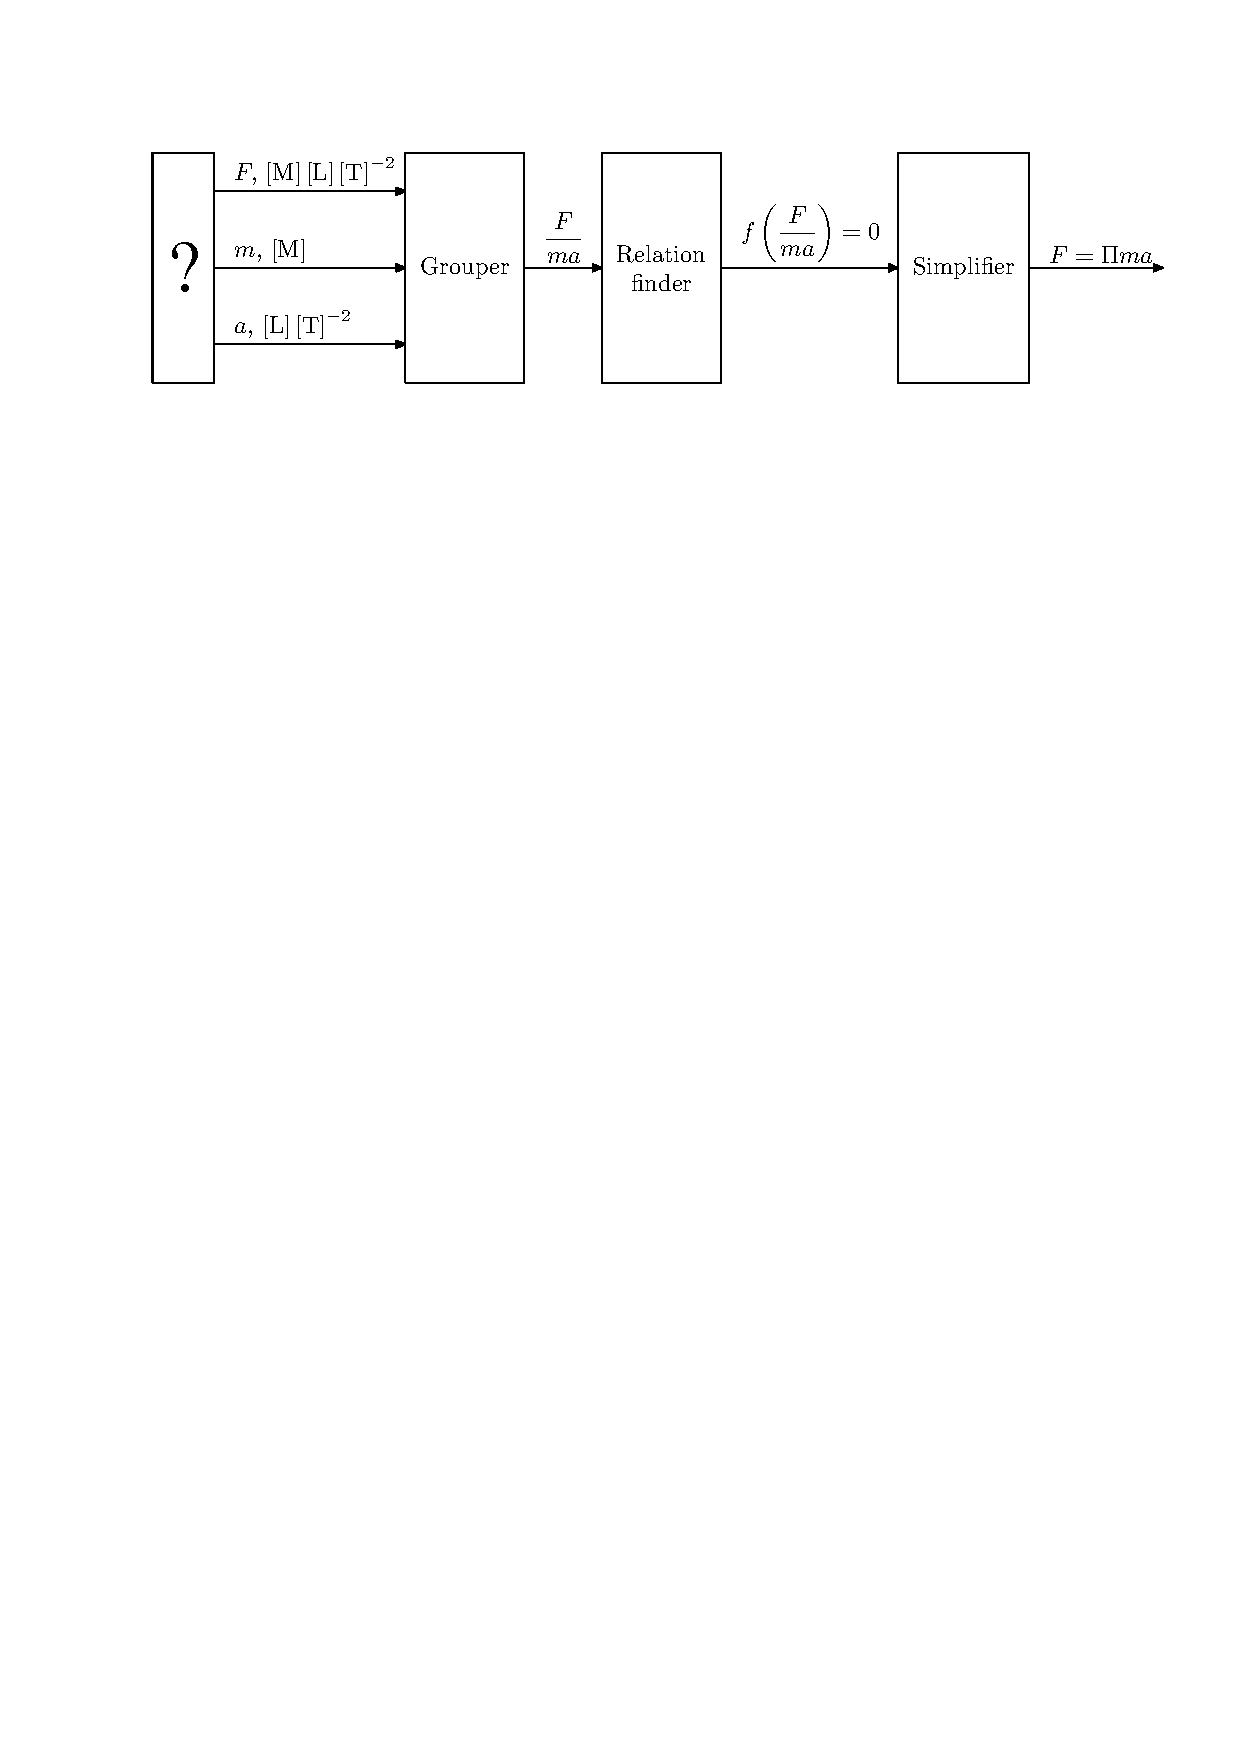
\includegraphics[width=0.9\textwidth]{./graphs/pi-machine.pdf}
\end{figure}
%%%
%
%
%%%
%
\begin{figure}[bt]\label{fig:solutionorder}
  \caption{As an example: the correct solution order for terminal velocity in turbulent flow. By starting in the \lingo{assume box}, we simplified the solution procedure. Step 1: On that assumption, we estimated the drag force (the \lingo{derive box}). Step 2: From the drag force, we estimated the terminal velocity (the \lingo{calculate box}). Step 3: From the terminal velocity, we estimated the Reynolds' number (the \lingo{check box}). Step 4: To close the loop, we verified the starting condition. Note: For compactness, the terminal-velocity formula ignores the normally small effect of buoyancy.}
  \centering
    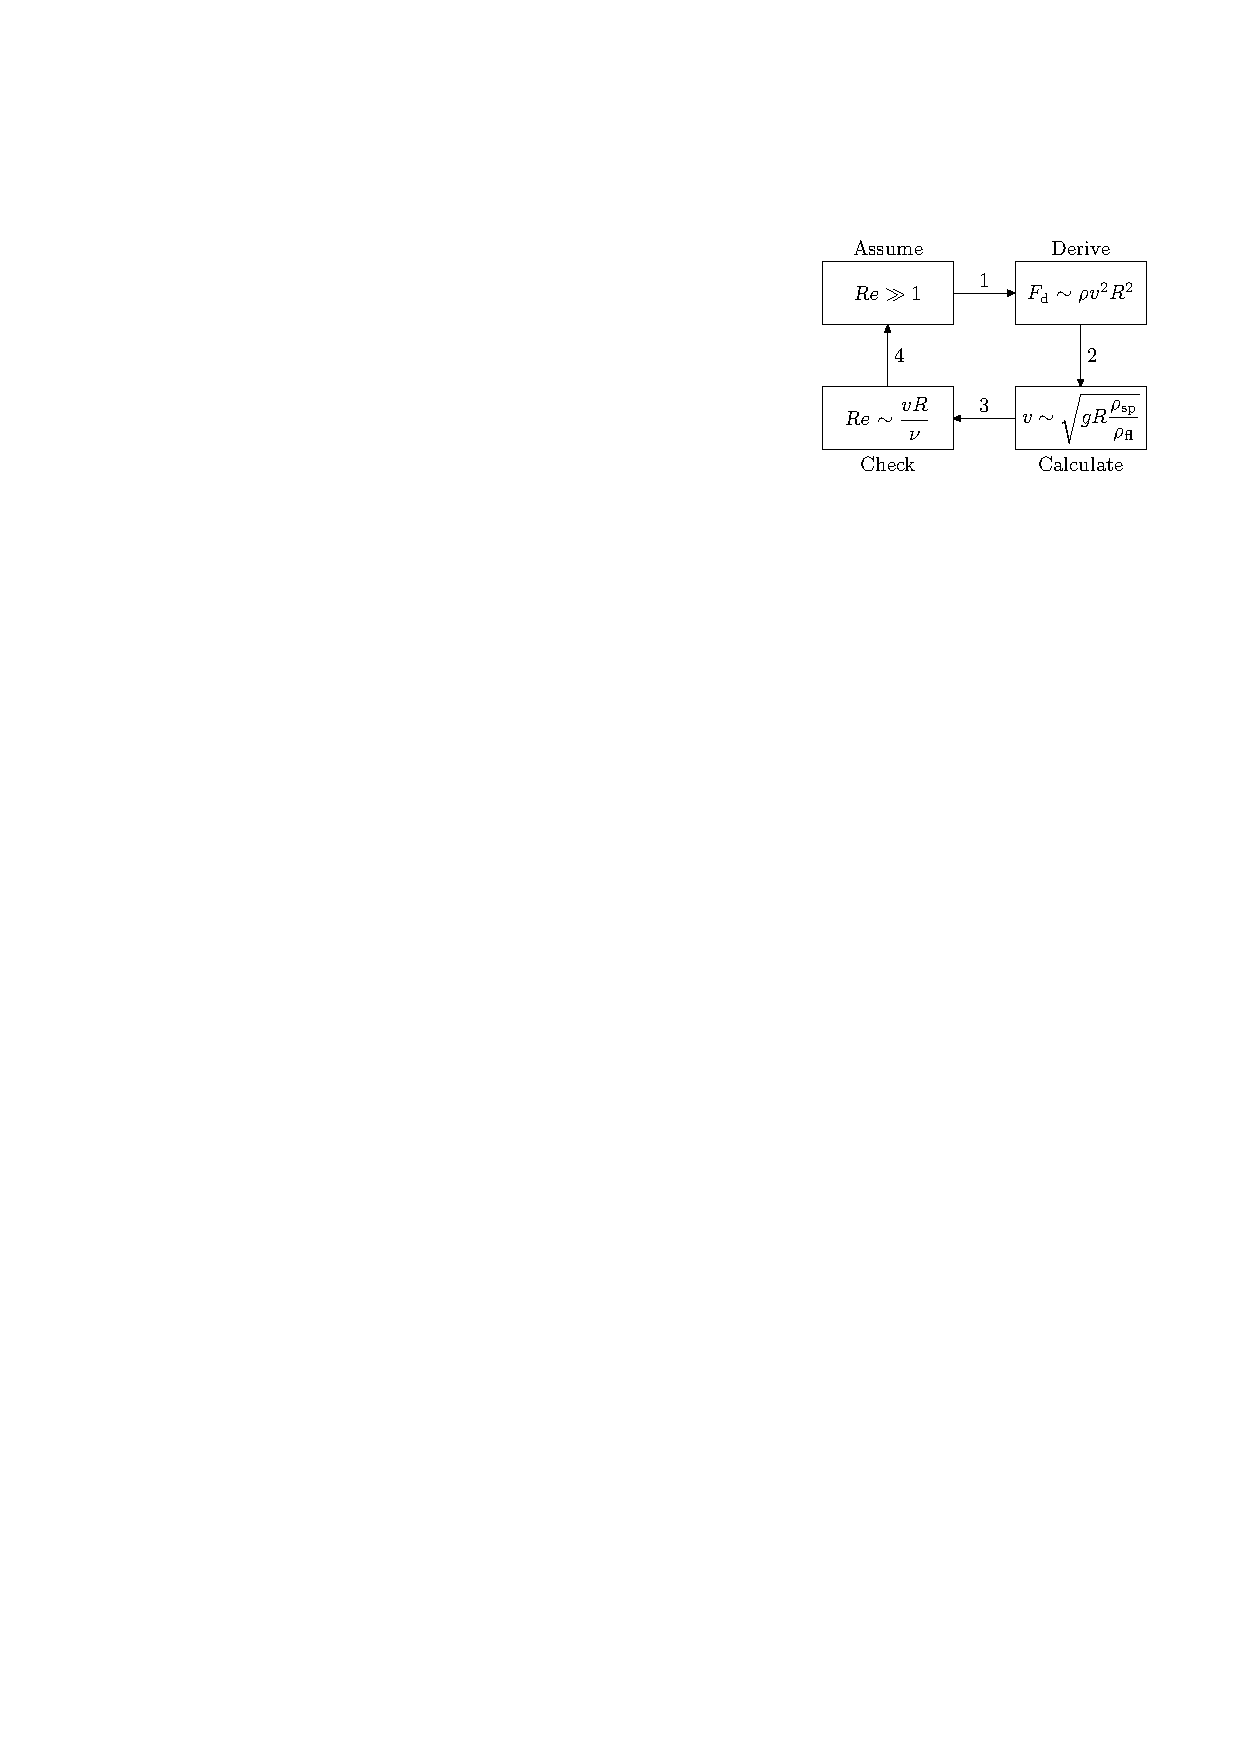
\includegraphics[width=0.5\textwidth]{./graphs/solution-order.pdf}
\end{figure}
%%%
%



\subsection{Nondimensionalization}
\lingo{Nondimensionalization} is the partial or full removal of physical dimensions from an equation involving physical quantities by a suitable substitution of variables. This technique can simplify and parameterize problems where measured units are involved. It is closely related to dimensional analysis. In some physical systems, the term scaling is used interchangeably with nondimensionalization, in order to suggest that certain quantities are better measured relative to some appropriate unit. These units refer to quantities intrinsic to the system, rather than units such as SI units. Nondimensionalization is not the same as converting extensive quantities in an equation to intensive quantities, since the latter procedure results in variables that still carry units.

Nondimensionalization can also recover characteristic properties of a system. For example, if a system has an intrinsic resonance frequency, length, or time constant, nondimensionalization can recover these values. The technique is especially useful for systems that can be described by differential equations. One important use is in the analysis of control systems. One of the simplest characteristic units is the doubling time of a system experiencing exponential growth, or conversely the half-life of a system experiencing exponential decay; a more natural pair of characteristic units is mean age/mean lifetime, which correspond to base $e$ rather than base 2.

Many illustrative examples of nondimensionalization originate from simplifying differential equations. This is because a large body of physical problems can be formulated in terms of differential equations. Consider the following:
\begin{itemize}
\item List of dynamical systems and differential equations topics
\item List of partial differential equation topics
\item Differential equations of mathematical physics
\end{itemize}

Although nondimensionalization is well adapted for these problems, it is not restricted to them. An example of a non-differential-equation application is dimensional analysis, while another is normalization in statistics.

Measuring devices are practical examples of nondimensionalization occurring in everyday life. Measuring devices are calibrated relative to some known unit. Subsequent measurements are made relative to this standard. Then, the absolute value of the measurement is recovered by scaling with respect to the standard.


\subsubsection{Rationale}
Suppose a pendulum is swinging with a particular period $T$. For such a system, it is advantageous to perform calculations relating to the swinging relative to $T$. In some sense, this is normalizing the measurement with respect to the period.

Measurements made relative to an intrinsic property of a system will apply to other systems which also have the same intrinsic property. It also allows one to \emph{compare a common property of different implementations of the same system}. Nondimensionalization determines in a systematic manner the \lingo{characteristic units} of a system to use, without relying heavily on prior knowledge of the system's intrinsic properties (one should not confuse characteristic units of a system with natural units of nature). In fact, \emph{nondimensionalization can suggest the parameters which should be used for analyzing a system}. However, it is necessary to start with an equation that describes the system appropriately.


\subsubsection{Nondimensionalization Steps}
To nondimensionalize a system of equations, one must do the following:
\begin{enumerate}
\item Identify all the independent and dependent variables;
\item Replace each of them with a quantity scaled relative to a characteristic unit of measure to be determined;
\item Divide through by the coefficient of the highest order polynomial or derivative term;
\item Choose judiciously the definition of the characteristic unit for each variable so that the coefficients of as many terms as possible become 1;
\item Rewrite the system of equations in terms of their new dimensionless quantities.
\end{enumerate}
The last three steps are usually specific to the problem where nondimensionalization is applied. However, almost all systems require the first two steps to be performed.

\begin{note}
Additionally, and more importantly, give a physical interpretation of the nondim. equation, of the nondim. quantities and of the characteristic quantities.
\end{note}


\begin{example}
Non-dimensionalize the following first order differential equation with constant coefficients:
\beq
a\xod x t + bx = A f\vat t\,.
\eeq
\end{example}

\begin{solution}
\begin{enumerate}
\item In this equation the independent variable here is $t$, and the dependent variable is $x$.
%
\item Set $x = \scpq x \chpq x$ and $t = \scpq t \chpq t$. This results in the equation
\beq
a\dfrac{\chpq x}{\chpq t}\xod{\scpq x}{\scpq t} + b \chpq x \scpq x = A f\vat{\scpq t \chpq t} \defby AF\vat{\scpq t}\,.
\eeq
%
\item The coefficient of the highest ordered term is in front of the first derivative term. Dividing by this gives
\beq
\xod{\scpq x}{\scpq t} + \dfrac{b\chpq t}{a}{\scpq x} = \dfrac{A\chpq t}{a\chpq x}F\vat{\scpq t}\,.
\eeq
%
\item The coefficient in front of $\scpq x$ only contains one characteristic variable $\chpq t$, hence it is easiest to choose to set this to unity first:
\beq
\dfrac{bt_c}{a} = 1 \implies \chpq t = \dfrac{a}{b}\,.
\eeq
Subsequently, 
\beq
\dfrac{A\chpq t}{a\chpq x} = \dfrac{A}{b\chpq x} = 1\implies \chpq x = \dfrac{A}{b}\,.
\eeq
%
\item The final dimensionless equation in this case becomes completely independent of any parameters with units:
\beq
\xod{\scpq x}{\scpq t} + \scpq x = F\vat{\scpq t}\,.
\eeq
\end{enumerate}
\end{solution}


\subsubsection{Substitutions}
Suppose for simplicity that a certain system is characterized by two variables -- a dependent variable $x$ and an independent variable $t$, where $x$ is a function of $t$, $x\vat t$. Both $x$ and $t$ represent quantities with units. To scale these two variables, assume there are two intrinsic units of measurement $\chpq x$ and $\chpq t$ with the same units as $x$ and $t$ respectively, such that these conditions hold:
\beq
\scpq t = \dfrac{t}{\chpq t}\implies t = \scpq t \chpq t\qquad\text{and}\qquad 
\scpq x = \dfrac{x}{\chpq x}\implies x = \scpq x \chpq x\,.
\eeq
These equations are used to replace $x$ and $t$ when nondimensionalizing. If differential operators are needed to describe the original system, their scaled counterparts become dimensionless differential operators.


\subsubsection{Conventions}
There are no restrictions on the variable names used to replace $x$ and $t$. However, they are generally chosen so that it is convenient and intuitive to use for the problem at hand. For example, if $x$ represented mass, the letter $m$ might be an appropriate symbol to represent the dimensionless mass quantity.

In this article, the following conventions have been used:
\begin{itemize}
\item $t$ represents the independent variable -- usually a time quantity. Its nondimensionalized counterpart is $\scpq t$.
\item $x$ represents the dependent variable -- can be mass, voltage, or any measurable quantity. Its nondimensionalized counterpart is $\scpq x$.
\end{itemize}

The subscripted $c$ added to a quantity's variable-name is used to denote the characteristic unit used to scale that quantity. For example, if $x$ is a quantity, then $\chpq x$ is the characteristic unit used to scale it.


\subsubsection{Differential Operators}
Consider the relationship:
\beq
              t = \scpq t\chpq t \implies \dx t = \chpq t\dx\scpq t \implies 
\xod{\scpq t} t = \dfrac{1}{\chpq t}\,.
\eeq

The dimensionless differential operators with respect to the independent variable becomes (the chain rule used)
\beq
\xod{}t  = \xod{\scpq t} t\xod{}{\scpq t} = \dfrac{1}{\chpq t}\xod{}{\scpq t}
\implies \nxod n{}t = \left(\xod{}t\right)^n
                    = \left(\dfrac{1}{\chpq t}\xod{}{\scpq t}\right)^n
                    = \dfrac{1}{\chpq t^n}\nxod n{}{\scpq t}\,.
\eeq


\subsubsection{Forcing Function}
If a system has a forcing function $f\vat t$, then
\beq
f\vat t = f\vat{\scpq t\chpq t} = f\vat{t\vat{\scpq t}} = F\vat{\scpq t}\,.
\eeq
Hence, the new forcing function $F$ is made to be dependent on the dimensionless quantity $\scpq t$.

\subsubsection{Linear Differential Equations with Constant Coefficients}

\subsubsection{First order system}
Let us consider the differential equation for a first order system:
\beq
a\xod xt + bx = Af\vat t\,.
\eeq
The derivation of the characteristic units for this system gives
\beq
\chpq t = \dfrac{a}{b}\qquad\text{and}\qquad\chpq x = \dfrac{A}{b} \,.
\eeq


\subsubsection{Second order system}
The second order system has the form
\beq
a\nxod 2xt + b\xod xt + cx = Af\vat t\,.
\eeq

Substitution step: Replace the variables $x$ and $t$ with their scaled quantities. The equation becomes
\beq
a\dfrac{\chpq x}{\chpq t^2}\nxod 2{\scpq x}{\scpq t}
  + b\dfrac{\chpq x}{\chpq t}\xod{\scpq x}{\scpq t}
  + c\chpq x\scpq t
  = Af\vat{\scpq t\chpq t} 
  = AF\vat{\scpq t}\,.
\eeq
This new equation is not dimensionless, although all the variables with units are isolated in the coefficients. Dividing by the coefficient of the highest ordered term, the equation becomes
\beq
\nxod 2{\scpq x}{\scpq t}
  + \chpq t\dfrac{b}{a}\xod{\scpq x}{\scpq t} 
  + \chpq t^2\dfrac{c}{a}\scpq x
  = \dfrac{A\chpq t^2}{a\chpq x}F\vat{\scpq t}\,.
\eeq
Now it is necessary to determine the quantities of $\chpq x$ and $\chpq t$ so that the coefficients become normalized. Since there are two free parameters, at most only two coefficients can be made to equal unity.

Determination of characteristic units: Consider the variable $\chpq t$:
\begin{itemize}
\item If $\chpq t = a/b$, then the first order term is normalized.
\item If $\chpq t^2 = a/b$, then the zeroth order term is normalized.
\end{itemize}
Both substitutions are valid. However, for pedagogical reasons, the latter substitution is used for second order systems. Choosing this substitution allows $\chpq x$ to be determined by normalizing the coefficient of the forcing function:
\beq
1 = \dfrac{A\chpq t^2}{a\chpq x} = \dfrac{A}{c\chpq x}\implies \chpq x = \dfrac{A}{c}
\eeq
The differential equation becomes
\beq
\nxod 2{\scpq x}{\scpq t} + \dfrac{b}{\sqrt{ac}}\xod{\scpq x}{\scpq t} + \scpq x = F\vat{\scpq t}\,.
\eeq
The coefficient of the first order term is dimentionless. Define
\beq
2\zeta \defby \dfrac{b}{\sqrt{ac}}\,.
\eeq
The factor 2 is present so that the solutions can be parameterized in terms of $\zeta$. In the context of mechanical or electrical systems, $\zeta$ is known as the \lingo{damping ratio} and is an important parameter required in the analysis of control systems. $2\zeta$ is also known as the \lingo{linewidth of the system}. The result of the definition is the \lingo{universal oscillator equation}.


\subsubsection{Mechanical Oscillations}
Suppose we have a mass attached to a spring and a damper, which in turn are attached to a wall, and a force acting on the mass along the same line. Define
\begin{itemize}
\item $x$ = displacement from equilibrium, $\phdim L$;
\item $t$ = time, $\phdim T$;
\item $F$ = external force or ``disturbance'' applied to system, , $\phdim{M.L/T^2}$;
\item $m$ = mass of the block, $\phdim M$;
\item $B$ = damping constant of dashpot, $\phdim{M/H}$;
\item $k$ = force constant of spring, $\phdim{M/T^2}$.
\end{itemize}
Suppose the applied force is a sinusoid $F = F_0\cos\vat{\omega t}$, the differential equation that describes the motion of the block is
\beq
m\nxod 2xt + B\xod xt + kx = F_0\cos\vat{\omega t}\,.
\eeq

Nondimensionalizing this equation the same way as described under second order system yields several characteristics of the system.

The intrinsic unit (characteristic quantity) $\chpq x$ corresponds to the \emph{distance} the block moves per unit force
\beq
\chpq x = \dfrac{F_0}{k}\,,
\eeq
the characteristic variable $\chpq t$ is equal to the \emph{period} of the oscillations
\beq
\chpq t = \sqrt{\dfrac{m}{k}}\,,
\eeq
and the dimensionless variable $2\zeta$ corresponds to the \emph{linewidth} of the system. $\zeta$ itself is the damping ratio
\beq
2\zeta = \dfrac{B}{\sqrt{mk}}\,.
\eeq


\subsubsection{Nonlinear Differential Equation}
Since there are no general methods of solving nonlinear differential equations, each case has to be considered on an individual basis when nondimensionalizing.

Quantum harmonic oscillator: The Schrödinger equation for the one dimensional time independent quantum harmonic oscillator is
\beq
\left( -\dfrac{\hbar^2}{2m}\nxod 2{}x + \dfrac{1}{2}m\omega^2 x^2 \right) \psi\vat x = E\psi\vat x\,.
\eeq
The modulus square of the wavefunction $\magn\psi^2$ represents probability, which is in a sense already dimensionless and normalized. Therefore, there is no need to nondimensionalize the wavefunction. However, it should be rewritten as a function of a dimensionless variable. Furthermore, the variable $x$ has dimensions of length. Hence substitute
\beq
\scpq x = \dfrac{x}{\chpq x}\qquad\text{and}\qquad \psi\vat x = \psi\vat{x\vat{\scpq x}} = \psi\vat{\scpq x}\,.
\eeq

The differential equation becomes
\begin{align*}
&\left(
  - \dfrac{\hbar^2}{2m\chpq x}\nxod 2{}{\scpq x} 
  + \dfrac{m\omega^2\chpq x^2}{2}\scpq x^2
\right) 
  \psi\vat{\scpq x}
  =
  E\psi\vat{\scpq x}\\
%
\implies &
%
\left(
  - \nxod 2{}{\scpq x} 
  + \dfrac{m^2\omega^2\chpq x^4}{\hbar^2}\scpq x^2
\right) 
  \psi\vat{\scpq x}
  =
  \dfrac{2Em\chpq x^2}{\hbar^2}\psi\vat{\scpq x}\,.
\end{align*}

To make the term in front of $\scpq x^2$ dimensionless, set
\beq
\dfrac{m^2\omega^2\chpq x^4}{\hbar^2} = 1\implies \chpq x = \sqrt{\dfrac{\hbar}{m\omega}}\,.
\eeq
Hence, the fully nondimensionalized equation is
\beq
\left(-\nxod 2{}{\scpq x} + \scpq x^2 \right)\psi\vat{\scpq x} 
    = \dfrac{2E}{\hbar\omega}\psi\vat{\scpq x}
    \defby \scpq{E}\psi\vat{\scpq x} \,. 
\eeq
The nondimensionalization factor for the energy is the same as the ground state of the harmonic oscillator. Usually, the energy term is not made dimensionless because a primary emphasis of quantum mechanics is determining the energies of the states of a system. Rearranging the first equation, the familiar equation for the harmonic oscillator is
\beq
\dfrac{\hbar\omega}{2}\left(-\nxod 2{}{\scpq x} + \scpq x^2 \right)\psi\vat{\scpq x}
    = E\psi\vat{\scpq x}\,.
\eeq


\subsection{Similitude}
\lingo{Similitude} is a concept applicable to the testing of engineering models. A model is said to have similitude with the real application if the two share geometric similarity, kinematic similarity and dynamic similarity. Similarity and similitude are interchangeable in this context.

The term dynamic similitude is often used as a catch-all because it implies that geometric and kinematic similitude have already been met.

Similitude's main application is in hydraulic and aerospace engineering to test fluid flow conditions with scaled models. It is also the primary theory behind many textbook formulas in fluid mechanics.


\subsubsection{Overview}
Engineering models are used to study complex fluid dynamics problems where calculations and computer simulations aren't reliable. Models are usually smaller than the final design, but not always. Scale models allow testing of a design prior to building, and in many cases are a critical step in the development process.

Construction of a scale model, however, must be accompanied by an analysis to determine what conditions it is tested under. While the geometry may be simply scaled, other parameters, such as pressure, temperature or the velocity and type of fluid may need to be altered. Similitude is achieved when testing conditions are created such that the test results are applicable to the real design.

The following criteria are required to achieve similitude:
\begin{itemize}
\item \lingo{Geometric similarity} -- The model is the same shape as the application, usually scaled.
%
\item \lingo{Kinematic similarity} -- Fluid flow of both the model and real application must undergo similar time rates of change motions. (fluid streamlines are similar)
%
\item \lingo{Dynamic similarity} -- Ratios of all forces acting on corresponding fluid particles and boundary surfaces in the two systems are constant.
\end{itemize}

To satisfy the above conditions the application is analyzed:
\begin{enumerate}
\item All parameters required to describe the system are identified using principles from continuum mechanics.
%
\item Dimensional analysis is used to express the system with as few independent variables and as many dimensionless parameters as possible.
%
\item The values of the dimensionless parameters are held to be the same for both the scale model and application. This can be done because they are dimensionless and will ensure dynamic similitude between the model and the application. The resulting equations are used to derive scaling laws which dictate model testing conditions.
\end{enumerate}

It is often impossible to achieve strict similitude during a model test. The greater the departure from the application's operating conditions, the more difficult achieving similitude is. In these cases some aspects of similitude may be neglected, focusing on only the most important parameters.

The design of marine vessels remains more of an art than a science in large part because dynamic similitude is especially difficult to attain for a vessel that is partially submerged: a ship is affected by wind forces in the air above it, by hydrodynamic forces within the water under it, and especially by wave motions at the interface between the water and the air. The scaling requirements for each of these phenomena differ, so models cannot replicate what happens to a full sized vessel nearly so well as can be done for an aircraft or submarine -- each of which operates entirely within one medium.

Similitude is a term used widely in fracture mechanics relating to the strain life approach. Under given loading conditions the fatigue damage in an un-notched specimen is comparable to that of a notched specimen. Similitude suggests that the component fatigue life of the two objects will also be similar.


\subsubsection{An Example}
Consider a submarine modeled at 1/40th scale. The application operates in sea water at \SI{0.5}{\celsius}, moving at \SI{5}{m/s}. The model will be tested in fresh water at \SI{20}{\celsius}. Find the power required for the submarine to operate at the stated speed.

A free body diagram is constructed and the relevant relationships of force and velocity are formulated using techniques from continuum mechanics. The variables which describe the system are:
\begin{itemize}
\item Variable -- Application -- Scaled mode -- Units
\item $L$ (diameter of submarine) -- 1 -- 1/40 -- \si{m}
\item $V$ (speed) -- 5 -- calculate -- \si{m/s}
\item $\rho$ (density) -- 1028 -- 998 -- \si{kg/m^3}
\item $\mu$ (dynamic viscosity) -- \num{1.88d-3} -- \num{1.00d-3} -- \si{Pa.s} or \si{N.s/m^2}
\item $F$ (force) -- calculate -- to be measured -- \si{N} or \si{kg.m/s^2}
\end{itemize}

This example has five independent variables and three fundamental units. The fundamental units are meter, kilogram, second.

Invoking the Buckingham $\pi$ theorem shows that the system can be described with two dimensionless numbers and one independent variable.

Dimensional analysis is used to re-arrange the units to form the Reynolds number $\rey$ and pressure coefficient $C\txt p$. These dimensionless numbers account for all the variables listed above except $F$, which will be the test measurement. Since the dimensionless parameters will stay constant for both the test and the real application, they will be used to formulate scaling laws for the test.

Scaling laws:
\begin{align*}
\rey &= \left(\dfrac{\rho V L}{\mu}\right) &\implies 
    V\txt m = V\txt a\left(\dfrac{\rho\txt a}{\rho\txt m}\right)\left(\dfrac{L\txt a}{L\txt m}\right)
              \left(\dfrac{\mu\txt m}{\mu\txt a}\right)\,,\\
%
C\txt p &= \left(\dfrac{2\diff p}{\rho V^2}\right)\,F = \diff pL^2 &\implies 
    F\txt m = F\txt a\left(\dfrac{\rho\txt a}{\rho\txt m}\right)\left(\dfrac{V\txt a}{V\txt m}\right)^2
              \left(\dfrac{L\txt a}{L\txt m}\right)^2\,.
\end{align*}
where the subscript $a$ stands for \emph{application} and $m$ for \emph{model}.

This gives a required test velocity of:
\beq
V\txt m = 21.9 V\txt a\,.
\eeq
The force measured from the model at that velocity is then scaled to find the force that can be expected for the real application:
\beq
F\txt a = 3.44 F\txt m\,.
\eeq
The power $P$ in watts required by the submarine is then:
\beq
P = F\txt a V\txt a = 17.2 F\txt m \,.
\eeq
Note that even though the model is scaled smaller, the water velocity needs to be increased for testing. This result shows how similitude in nature is often counter-intuitive.


\subsubsection{Typical applications}
Similitude has been well documented for a large number of engineering problems and is the basis of many textbook formulas and dimensionless quantities. These formulas and quantities are easy to use without having to repeat the laborious task of dimensional analysis and formula derivation. Simplification of the formulas (by neglecting some aspects of similitude) is common, and needs to be reviewed by the engineer for each application.

Similitude can be used to predict the performance of a new design based on data from an existing, similar design. In this case, the model is the existing design. Another use of similitude and models is in validation of computer simulations with the ultimate goal of eliminating the need for physical models altogether.

Another application of similitude is to replace the operating fluid with a different test fluid. Wind tunnels, for example, have trouble with air liquefying in certain conditions so helium is sometimes used. Other applications may operate in dangerous or expensive fluids so the testing is carried out in a more convenient substitute.

Some common applications of similitude and associated dimensionless numbers:
\begin{itemize}
\item Incompressible flow: Reynolds number, Pressure coefficient, Froude number and Weber number for open channel hydraulics;
%
\item Compressible flows: Reynolds number, Mach number, Prandtl number, Specific heat ratio;
%
\item Flow-excited vibration: Strouhal number;
%
\item Centrifugal compressors: Reynolds number, Mach number, Pressure coefficient, Velocity ratio;
%
\item Boundary layer thickness: Reynolds number, Womersley number, Dynamic similarity.
\end{itemize}


\subsection{Economy of Graphical Representation}

\epigraph{A good table of functions of one variable may require a page; that of a function of two variables a volume; that of a function of three variables a bookcase; and that of a function of four variables a library.}
{Harold Jeffreys}{quoted in Street-Fighting Mathematics}

One of the most significant benefits of using dimensionless versus physical variables is the very substantial saving of space and effort in the logistic in presenting the relations graphically. To illustrate, suppose we wish to find from a chart the dependent variable for $k$ distinct values of the independent variable and the $p$ number of parameters, each of which can also assume $k$ distinct values. To present such a function graphically, how many curves do we need? The answer is found by the following simple argument:
\begin{itemize}
\item if there are zero parameters, then we need $k^0 = 1$ curves;
\item if there is one parameter, then we need $k^1 = k$ curves;
\item if there are two parameters, then we need $k^2$ curves;
\item so, in general, if there are $p$ parameters, then we need $k^p$ curves.
\end{itemize}
The last generalization can be written as
\beq
N\txt{curves} = k^p\,,
\eeq
where $N\txt{curves}$ represents the number of curves needed to present the given relationship, $k$ the number of distinct values for the dependent variable and each parameter and $p$ the number of parameters.

If $N\txt{var}$ is the number of variables, then the number of parameters is generally
\beq
p = N\txt{var} - 2\,,
\eeq
since we consider \emph{one} variable to be independent and \emph{one} dependent. Thus, by plugging the last equation into the number of curves one has
\beq
N\txt{curves} = k^{N\txt{var} - 2}\,,
\eeq

A chart can have one \lingo{family of curves} characterized by a single \lingo{parameter}. Thus, each curve has a particular value of this parameter assigned to it, and therefore there are $k$ curves in a chart. It follows that the number of charts required to present a relation of $N\txt{var}$ variables is
\beq
\begin{cases}
N\txt{chart} = k^{N\txt{var} - 3} \quad\text{if $N\txt{var} > 2$}\,,\\
N\txt{chart} = 1                  \quad\text{if $N\txt{var} = 2$}\,.
\end{cases}
\eeq

One can see from these equations that the number of curves and charts to be plotted grows rather vehemently with the number of variables -- so much so that the situation soon becomes unmanageable. Is there a way out of this predicament? Yes, there is, use dimensionless variables!

As seen from the Buckingham Pi Theorem:
\beq
N\txt{dimless} = N\txt{var} - N\txt{dims}\,,
\eeq
where $N\txt{dimless}$ is the number of dimensionless variables which can be formed from (and by) $N\txt{var}$ number of physical variables and $N\txt{dims}$ is the number of dimensions.

Here we assumed that the rank of the dimensional matrix is not less than the number of dimensions $N\txt{dims}$. If this condition is not fulfilled, then we must delete one or more dimensions to gain the equality of $N\txt{dims}$ with the rank of dimensional matrix.

So, if we have $N\txt{dims}$ dimensions in a relation, then the number of dimensionless variables that can be formed is always less than the number of variables in that relation. This results in a very significant improvement in the logistics of graphical presentation. If we substitute $N\txt{dimless}$ for $N\txt{var}$, we obtain
\beq
\begin{cases}
N'\txt{curve} = k^{N\txt{var} - N\txt{dim} - 2}\,,\\
N'\txt{chart} = k^{N\txt{var} - N\txt{dim} - 3}\,.
\end{cases}
\eeq
Hence,
\beq
z = \dfrac{N\txt{curve}}{N'\txt{curve}} = \dfrac{N\txt{chart}}{N'\txt{chart}}\,.
\eeq
Note that this ratio is \emph{independent} of the number of variables and is dependent only upon the number of dimensions $N\txt{dim}$ and the number of distinct values $k$ for each parameter. For example, if we have a relation of three dimensions and six distinct values for each parameter (variable), then by \emph{not} employing dimensionless variables, we would need $z = k^{N\txt{dim}} = 63 = 216$ times as many curves and charts as we would if we used only these variables.

Example: Gravitational Acceleration on a Celestial Body as a Function of Altitude (Positive or Negative):

\begin{solution}
To find the altitude-dependent gravitational acceleration on a celestial body, we deal with the following variables:
\begin{itemize}
\item gravitational acceleration, $g$, $\si{m/s^2}$;
\item distance from center of the celestial body, $R$, $\si{m}$;
\item universal gravitational const., $G$, $\si{m^3/(kg.s^2)}$; 
\item mass of celestial body, $M$, $\si{kg}$;
\item radius of celestial body, $R_0$, $\si{m}$.
\end{itemize}
We have five variables and hence, if the number of distinct values of variables is $k = 6$, then to represent the relation $g = \Phi\vat{R, G, M, R_0}$ graphically, we need 216 curves drawn on 36 charts. What do we have if we use dimensionless variables? There are five variables and three dimensions, therefore we have $5 - 3 = 2$ dimensionless variables, from which we can find the dimensionless quantities
\beq
\kdim_1 = \dfrac{gR_0^2}{GM} \qquad\text{and}\qquad
\kdim_2 = \dfrac{R}{R_0}\,.
\eeq
So now we have only \emph{two} (dimensionless) variables and, therefore, the relation can be plotted by a \emph{single} curve -- a 216-fold improvement!

To continue now, we can write
\beq
\kdim_1 = \Phi\vat{\kdim_2}\,,
\eeq
which, by assuming monomial form, can be written
\beq
\kdim_1 = c\kdim_2^n\,,
\eeq
where $c$ and $n$ are pure numbers still to be determined. As a simple analytic derivation (not presented here) can show, $c = 1$ and 
\beq
\begin{cases}
n = -2 \qquad\text{if $R > R_0$}\,,\\
 n = 1 \qquad\text{if $R < R_0$}\,.
\end{cases}
\eeq
Fig. [...] (graph: in $x$-axis $\kdim_2$ and in $y$-axis $\kdim_1$, because the relation is $\kdim_1 = \Phi\vat{\kdim_2}$) presents this ``one-curve'' plot. Note the interesting feature that $n$ is not constant but varies -- rather abruptly -- with the sign of the altitude. The plot shows that $g$ is maximum at ``sea level'' on any homogeneous celestial body.
\end{solution}


\subsection{Steps of Dimensional Analysis}

[Qing-Ming Tan, dim analysis with case studies in mechanics]

The principles of dimensional analysis provide the only way to solve complex problems when there is no available mathematical model. To deal with such problems, it is natural for me to apply the steps of dimensional analysis:
\begin{itemize}
\item Analyze physical effects involved in the problem. 
\item Select corresponding governing parameters.
\item Design experiments.
\item Analyze and synthesize experimental data.
\item Establish dimensionless relationships between cause and effect parameters.
\end{itemize}


\subsection{Steps of Dimensional Analysis -- Again}
Use the following procedure to perform dim. analysis:
\begin{itemize}
\item Identify the problem domain: geometry, mechanics, thermal energy transfer, mass transfer and so on.
%
\item Choose a dim-independent set of physical quantities accordingly to the problem domain: $\elset{L}$, $\elset{L,T}$, $\elset{M,L,T}$, $\elset{F,L,T}$, $\elset{E,L,T,\Theta}$ and so forth. Count the elements as $m$.
%
\item Identify the transport properties (fluid velocity, thermal flux, mass flux, ...) and the material properties (viscosity, thermal conduction, density, specific thermal capacity, ...). Count all the properties as $n$. (Do \emph{not} forget to include the quantity being sought!)
%
\item Define the dimensions of all the properties in the dim-ind system.
%
\item Calculate the number of dimensionless quantities: $r = n - m$.
%
\item Form the dimless quantities: $\kdim_i$. (The first one, $\kdim_1$, should be the one containing the quantity being sought!)
%
\item Apply the principle of dimensional homogeneity of physical laws:
\beq
f\vat{\kdim_i} = 0\,.
\eeq
%
\item Classify the different dimensionless quantities and give them physical interpretation.
%
\item When possible, use physical information, intuition or approximate methods (simplification, extreme cases, ...) to reduce the number of dimless quantities.
%
\item If required make experiments to find the functional form of $f$.
%
\item Make calculations with the final form of $f$ in order to obtain numerical values that can be used to review assumptions, simplifications, approximations, \etc.
\end{itemize}


\subsection{Examples}

\subsubsection{Nondimensionalized the equation of motion for a simple pendulum.}

The motion of a simple pendulum is modeled using the following (ordinary) differential equation and boundary and initial conditions:
\beq
\begin{cases}
\nxod 2\phi t = -\dfrac{g}{l}\sin\vat\phi\,,\\
       \phi_0 = \phi\vat 0\,,\\
   \xod\phi t = 0\,.
\end{cases}
\eeq

To non-dim. the equation of motion, follow the five-step method:
\begin{enumerate}
\item the independent variable is $t$, whereas the dependent one is $\phi$.
%
\item $\phi$ is already dimensionless, so nothing to do here. For $t$, find the characteristic time $\chpq t$ as $t = \chpq t\scpq t$, where $\scpq t$ is the scaled (dimensionless) time. With this replacement, find the derivatives
\beq
      t = \chpq t\scpq t \implies 
  \dx t = \chpq t\dx \scpq t \implies 
\dx t^2 = \chpq t^2\dx \scpq t^2\,.
\eeq
%
\item Replace the scaled variables and their derivatives in the original differential equation and boundary and initial conditions
\beq
\begin{cases}
\dfrac{1}{\chpq t^2}\nxod 2{\phi}{\scpq t} + \dfrac{g}{l}\sin\vat\phi = 0 \implies
    \nxod 2{\phi}{\scpq t} + \dfrac{g\chpq t^2}{l}\sin\vat\phi = 0\,,\\
%
\phi_0 = \phi\vat 0\,,\\
%
\dfrac{1}{\chpq t}\xod{\phi}{\scpq t} = 0 \implies
    \xod{\phi}{\scpq t} = 0\,.
\end{cases}
\eeq
%
\item In the non-dim. model differential equation, the coefficient in front of $\sin\vat\phi$ has only one characteristic quantity: $\chpq t$. So set it to unity to find
\beq
\dfrac{g\chpq t^2}{l} = 1 \implies \chpq t = \sqrt{\dfrac{l}{g}}\,.
\eeq
Note that $\chpq t$ equals $\sqrt{l/g}$, which, in turn, equals the pendulum period. In other words, the pendulum period is a characteristic quantity: the period is the pendulum's own clock!
%
\item With these changes, the model becomes finally
\beq
\begin{cases}
\nxod 2{\phi}{\scpq t} + \sin\vat\phi = 0\,,\\
\phi_0 = \phi\vat 0\,,\\
\xod{\phi}{\scpq t} = 0\,.
\end{cases}
\eeq
Not only is this final equation, and its boundary and initial conditions, dimensionless, but also parameter-free!
%
\end{enumerate}

An analytic solution to the pendulum equation can be found by considering small swings, where the approximation $\sin\vat\phi\sim\phi$ is valid. The equation for the model thus becomes
\beq
\nxod 2\phi t + \dfrac{g}{l}\phi = 0\,.
\eeq
After integration and replacement of boundary and initial conditions, one finds
\beq
\phi = \phi_0\cos\vat{t/\sqrt{l/g}}\,.
\eeq
Note that the argument of the cosine function is dimensionless and equals the pendulum period; \ie, as expected, the model was dimensionless all along!


\subsubsection{Nondimensionalized the equation of motion for a vertical projectile.}
Suppose that a projectile of mass $m$ is thrown vertically into the air with an initial velocity $v_0$.

Note by $x$ the position of the projectile at any time $t$. Then, the equations of motion for the projectile are
\beq
\begin{cases}
    m\ddt x = -mg\,,\\
    x\vat 0 = 0\,,\\
\dt x\vat 0 = v_0\,.
\end{cases}
\eeq
In this set of equations, the independent quantity is $t$, the dependent one $x$ and the parameters $g$ and $v_0$.

Choose the characteristic quantities for the phenomenon by
\begin{align*}
\scpq x &= x/\chpq x\implies x = \chpq x\scpq x\,,\\
%
\scpq t &= x/\chpq t\implies t = \chpq t\scpq x\implies \dx t = \chpq t\dx{\scpq t}\implies \dx t^2 = \chpq t^2\dx{\scpq t}^2\,.
\end{align*}
With these choices, the equations of motion become
\beq
\begin{cases}
\dfrac{\scpq x}{\scpq t^2}\nxod{2}{\scpq x}{\scpq t} = -g\,,\\
x\vat 0 = 0 \implies \scpq x\vat 0 = 0\,,\\
\dfrac{\scpq x}{\scpq t}\xod{\scpq x}{\scpq t}\vat 0 = v_0\,.
\end{cases}
\eeq

Noting that $\dim v_0^2/g = \phdim L$ and that $\dim v_0/g = \phdim T$, find $\chpq x$ and $\chpq t$ by
\beq
\chpq x = \dfrac{v_0^2}{g}\qquad\text{and}\qquad
\chpq t = \dfrac{v_0}{g}\,.
\eeq

Replace $\chpq x$ and $\chpq t$ in the equations of motion to have
\beq
\begin{cases}
\dfrac{v_0^2}{g}\dfrac{g^2}{v_0^2}\nxod{2}{\scpq x}{\scpq t} = -g\implies \nxod{2}{\scpq x}{\scpq t} = -1\,,\\
\scpq x\vat 0 = 0\,,\\
\dfrac{v_0^2}{g}\dfrac{g}{v_0}\xod{\scpq x}{\scpq t}\vat 0 = v_0\implies \xod{\scpq x}{\scpq t}\vat 0 = 1\,.
\end{cases}
\eeq

Finally, write the equations of motion as
\beq
\nxod{2}{\scpq x}{\scpq t} = -1\,,\qquad
\scpq x\vat 0 = 0\qquad\text{and}\qquad
\xod{\scpq x}{\scpq t}\vat 0 = 1\,.
\eeq
Note that the last set of equations is dimensionless and parameter free!


\subsubsection{Nondimensionalized the equation of motion for a vertical projectile -- again}
Suppose that a projectile of mass $m$ is thrown vertically into the air with an initial velocity $v_0$.

The modeling equations for the particle motion for this system are:
\beq
\begin{cases}
\nxod 2xt = -g\,\\
  x\vat 0 = 0\,\\
  \xod xt = v_0\,.
\end{cases}
\eeq

The independent variable is $t$, the dependent one is $x$ and the parameters are $g$ and $v_0$.

Choose the characteristic and scaled quantities by
\begin{align*}
& x = \chpq x\scpq x \implies \dx x = \chpq x\dx\scpq x \implies \dx^2x = \chpq x\dx^2\scpq x\,,\\
& t = \chpq t\scpq t \implies \dx t = \chpq t\dx\scpq t \implies \dx t^2 = \chpq t^2\dx \scpq t^2\,.
\end{align*}

Replace the chosen quantities in the physical model:
\begin{align*}
\dfrac{\chpq x}{\chpq t^2}\nxod 2{\scpq x}{\scpq t} &= -g\,,\\
\chpq x\scpq x\vat 0 &= 0\implies \scpq x\vat 0 = 0\,,\\
\dfrac{\chpq x}{\chpq t}\xod{\scpq x}{\scpq t}\vat 0 &= v_0\,.
\end{align*}

Manipulate the last set of equations to have
\begin{align*}
\nxod 2{\scpq x}{\scpq t} &= -\dfrac{g\chpq t^2}{\chpq x}\,,\\
\chpq x\scpq x\vat 0 &= 0\implies \scpq x\vat 0 = 0\,,\\
\xod{\scpq x}{\scpq t}\vat 0 &= \dfrac{\chpq t v_0}{\chpq x}\,.
\end{align*}

Equate the coefficients of the RHSs of the last equations to unity
\beq
 \dfrac{g\chpq t^2}{\chpq x} = 1\qquad\text{and}\qquad
\dfrac{\chpq t v_0}{\chpq x} = 1\,,
\eeq
to find that
\beq
\chpq x = \dfrac{v_0^2}{g}\qquad\text{and}\qquad
\chpq t = \dfrac{v_0}{g}\,.
\eeq

Replace the characteristic quantities into the set of equations for the model to have
\begin{align*}
\nxod 2{\scpq x}{\scpq t} &= -\dfrac{v_0^2/g^2}{v_0^2/g}g = -1\,,\\
\scpq x\vat 0 &= 0\,,\\
\xod{\scpq x}{\scpq t}\vat 0 &= \dfrac{v_0/g}{v_0^2/g}v_0 = 1\,.
\end{align*}

This replacements leave the final set of equations for the model:
\begin{align*}
\nxod 2{\scpq x}{\scpq t} &= -1\,,\\
\scpq x\vat 0 &= 0\,,\\
\xod{\scpq x}{\scpq t}\vat 0 &= 1\,.
\end{align*}

To go back to the original, dimensional, physical quantities, the transformation equations are
\begin{align*}
x &= \chpq x\scpq x \implies \scpq x = x/\chpq x = x/(v_0^2/g) = gx/v_0^2\,,\\
t &= \chpq t\scpq t \implies \scpq t = t/\chpq t = t/(v_0/g) = gt/v_0\,. 
\end{align*}
